\cleardoublepage
\section{Tính giá trị điện áp tại $V_{C2}$ và điện trở 20ohm tự chọn transistor và zenner để mô phỏng, so sánh kết quả}
    \subsection{Hình a}
    \subsubsection{Tính $V_{C2}$}
    \begin{figure}[H]
        \centering
        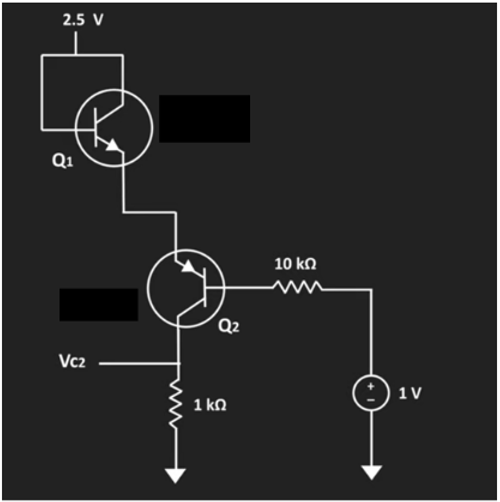
\includegraphics[width=0.5\textwidth]{pictures/topic5_a.png}
        \caption{Đề bài a}					
    \end{figure}
    Chọn $V_{BE1} = V_{BE2}$ theo số liệu transistor NPN trong proteus \\
    $\Rightarrow V_{BE1} = V_{BE2} = 0.73777V$ và $\beta _1 = \beta _2 = 100$\\
    \begin{itemize}
        \item $V_{B1} = 2.5V$
        \item $V_{E1} = V_{B1} - 0.73777 = 1.76223V$
    \end{itemize}
    \[
    \begin{cases}
        V_{E2} = V_{B2} + 0.73777 \\
        V_{E2} = V_{E1}
    \end{cases}
    \]
    \[
        \Rightarrow V_{B2} = 1.02446V
    \]
    \begin{itemize}
        \item $\frac{V_{B2}-1}{10} = I_{B2} \Rightarrow I_{B2} = 0.002446(mA)$  
        \item $I_{C2} = \beta _2 I_{B2} = 100*0.002446 = 0.2446 (mA)$ 
        \item $V_{C2} = I_{C2}.1k\Omega  = 0.2446*1000 = 0.2446 (V)$
    \end{itemize}
    \subsubsection{Kiểm tra bằng proteus}
    \begin{figure}[H]
        \centering
        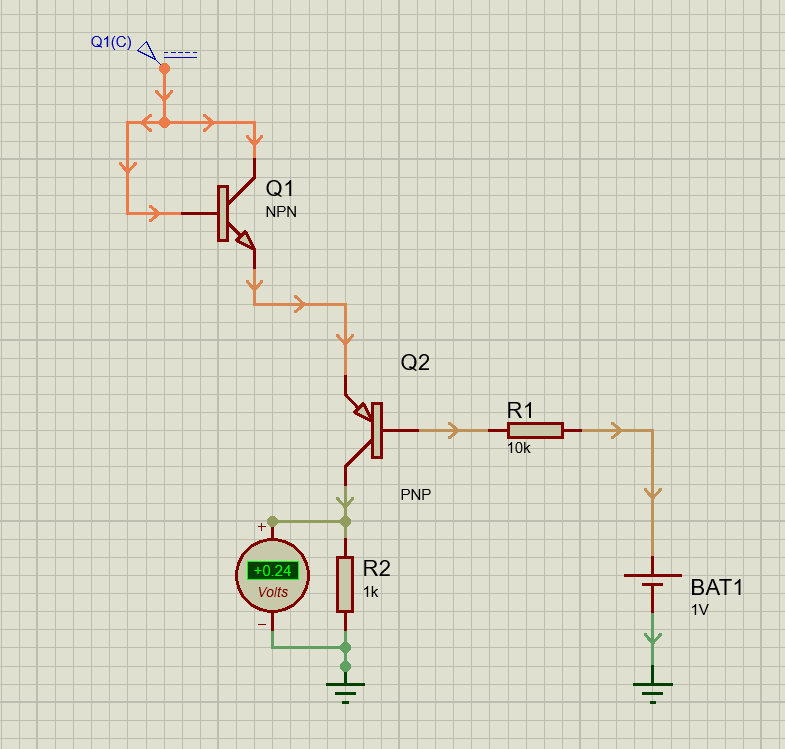
\includegraphics[width=0.7\textwidth]{pictures/result5_a.png}
        \caption{Mô phỏng mạch a bằng proteus}
    \end{figure}
    $\Rightarrow$ \textbf{Mô phỏng proteus cho kết quả giống với giá trị đã tính toán được trước đó.}\\
    \cleardoublepage
    \subsection{Hình b}
    \subsubsection{Tính toán}
    \begin{figure}[H]
        \centering
        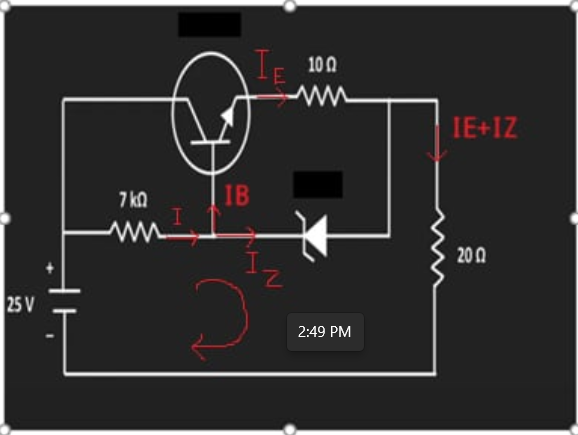
\includegraphics[width=0.8\textwidth]{pictures/pic5_b.png}
        \caption{Đề bài b}
    \end{figure}
    Chọn $\beta$ = 100; diode zenner: 4.7V (1N4732A)
    \begin{itemize}
        \item $I_E = \frac{4.7 - 0.7}{10} = 0.4 \rightarrow I_B = \frac{I_E}{\beta} = 0.004$
        \item $I = I_B + I_2$
    \end{itemize}
    Áp dụng định luật Kiffchoff:
    \[
        25 = 7*10^3(I_B + I_2) + 4.7 + 20(I_E + I_2)\\
    \]
    \[
        \Longleftrightarrow 25 = 7*10^3(0.004 + I_2) + 4.7 + 20(0.4 + I_2) \\
    \]
    \[
        \rightarrow 25 = 28 + 7000I_2 + 4.7 + 8 + 20I_2 \\
    \]
    \[
        \rightarrow I_2 = \frac{25 - 28 - 4.7 - 8}{7020} = -0.002 < 0\\
    \]
    $\Rightarrow$ Không có dòng qua diode\\
    Áp dụng định luật Kiffchoff:
    \[
    \begin{cases}
        25 = 7*10^3*I_B + I_E*10 + I_E*20\\
        I_E = 100I_B\\
    \end{cases} 
    \]
    \[
    \Rightarrow 25 =7*10^3\frac{I_E}{100} + 10I_E + 20 I_B\\
    \]
    \[
    \Rightarrow I_E = \frac{25}{100} = 0.25 A\\
    \]
    \[
    \Rightarrow V_{R_{20\Omega }} = 0.25*20 = 5V\\
    \]
    \subsubsection{Kiểm tra bằng proteus}
    \begin{figure}[H]
        \centering
        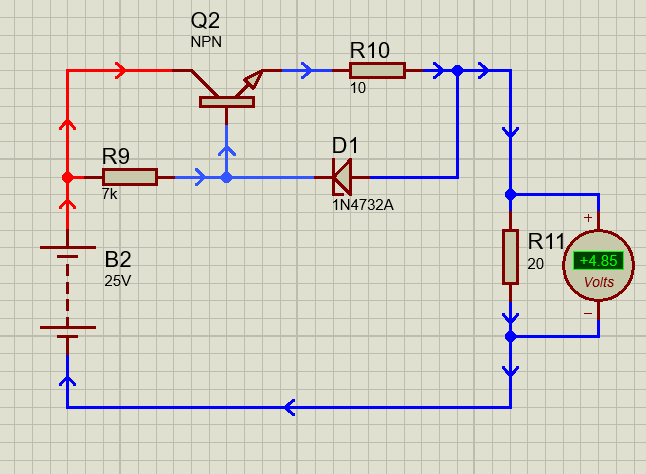
\includegraphics[width=0.8\textwidth]{pictures/result5_b.png}
        \caption{Mô phỏng mạch bằng proteus}
    \end{figure}
    $\Rightarrow$ 
    \textbf{Kết quả mô phỏng bằng proteus cho thấy giá trị điện áp tại $V_{R_{20\Omega }}$ là 4.85V, tương đối chính xác với sai lệch 0.15V. Điều này xảy ra do làm tròn trong lúc tính toán và chọn $\beta$.}
